We created a tool, OptiFuzz, that can be used to generate, fuzz and analyze random C programs.
The source code for OptiFuzz is available on GitHub\footnote{\url{https://github.com/anbclausen/optifuzz}.}.
The goal of OptiFuzz is to quantify the issue of timing attacks introduced by C compilers with different optimization flags enabled.
The tool works as follows:
\begin{itemize}
  \item OptiFuzz generates random C programs consisting of non-branching arithmetic, logical and comparison operations.
  \item OptiFuzz then compiles the generated C programs with different specified optimization flags enabled and inspects the generated assembly for conditional branching instructions introduced by the compiler.
        If branching is found, the program is flagged.
  \item OptiFuzz then fuzzes the flagged programs with various random inputs to test whether the branching instructions can be exploited to leak information about the input.
  \item At last, OptiFuzz applies Welch's t-test on the fuzzing data to detect whether a timing vulnerability is present.
        Furthermore, OptiFuzz reports the results of the fuzzing in the form of a PDF report.
\end{itemize}
The OptiFuzz pipeline is illustrated in Figure \ref{fig:optifuzz-pipeline}. 
Each of the steps in the pipeline is described in detail in the following sections.
\begin{figure}[H]
  \centering
  \tikzstyle{box} = [rectangle, minimum width=3cm, minimum height=1cm, text centered, draw=black]
\tikzstyle{arrow} = [thick,->,>=stealth]

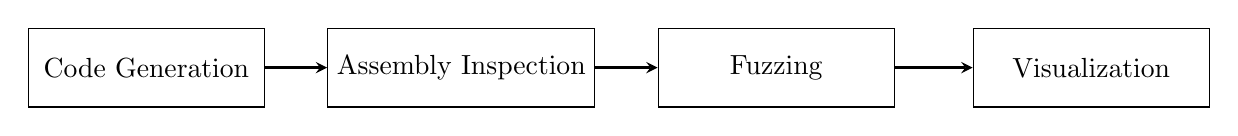
\begin{tikzpicture}
  \node (Code Generation) [box] {Code Generation};
  \node (Assembly Inspection) [box, right of=Code Generation, xshift=3cm] {Assembly Inspection};
  \node (Fuzzing) [box, right of=Assembly Inspection, xshift=3cm] {Fuzzing};
  \node (Visualization) [box, right of=Fuzzing, xshift=3cm] {Visualization};

  \draw [arrow] (Code Generation) -- (Assembly Inspection);
  \draw [arrow] (Assembly Inspection) -- (Fuzzing);
  \draw [arrow] (Fuzzing) -- (Visualization);
\end{tikzpicture}
  \caption{The OptiFuzz pipeline.}
  \label{fig:optifuzz-pipeline}
\end{figure}
